\chapter{Mérési eredmények}
%%%%%%%%%%%%%%%%%%%%%%%%%%%%%%%%%%%%%%%%%%%%%%%%%
%(12-15 oldal)



%\section{Mérési eredmények}
%(7-10 oldal): kinyert mérések tartalma(delay, jitter, link, AS info, Geolocation), mérések mennyisége, mérések minősége

\section{Létrehozott adatbázis bemutatása}
Jelen fejezet bemutatja a létrehozott adatbázis fontosabb adathalmazait, amelyek további elemzések alapját képezi.

\subsection*{Éllista}
A legfontosabb eredmény az internetes útvonalakat alkotó gépek közötti kapcsolatokról szolgáltat mérési eredményeket. Az objektum amelyről a mérés készült egy internetes link, a kinyert információk a következők:

\begin{itemize}
\item \textbf{delay:} Késleltetés a két gép közötti kapcsolaton (két gép közötti elméleti rtt)
\item \textbf{rtt:} A from számítógéphez végzett körülfordulási idő a mérést végző measurer\_ip számítógéptől
\item \textbf{time:} A mérés időpontja
\item \textbf{jitter:} Késleltetés ingadozás a két számítógép között
\item \textbf{measurer\_ip:} A mérést végző számítógép (ahol a traceroute parancs fut)
\item \textbf{target\_ip:} Az útvonalmérés célpontja
\item \textbf{to:} A linkek a mérést végző számítógéptől távolabbi csomópontjának információi: city, country, longitude, latitude, ip, asn
\item \textbf{from:} A linknek a mérést végző számítógéphez közelebbi csomópontjának információi: city, country, longitude, latitude, ip, asn
\end{itemize}



Az elkészült mérési rendszernek ez az adat kollekció\footnote{A MongoDB adatbázisban táblák helyett kollekciókban tárolódnak az adatbejegyzések} az egyik legfontosabb eredménye. A Traceroute parancs futtatásának kimenetéből lett feldolgozva\cite{traceParse} és további adatmezőkkel felgazdagítva.

\begin{figure}[h!]
	\centering
	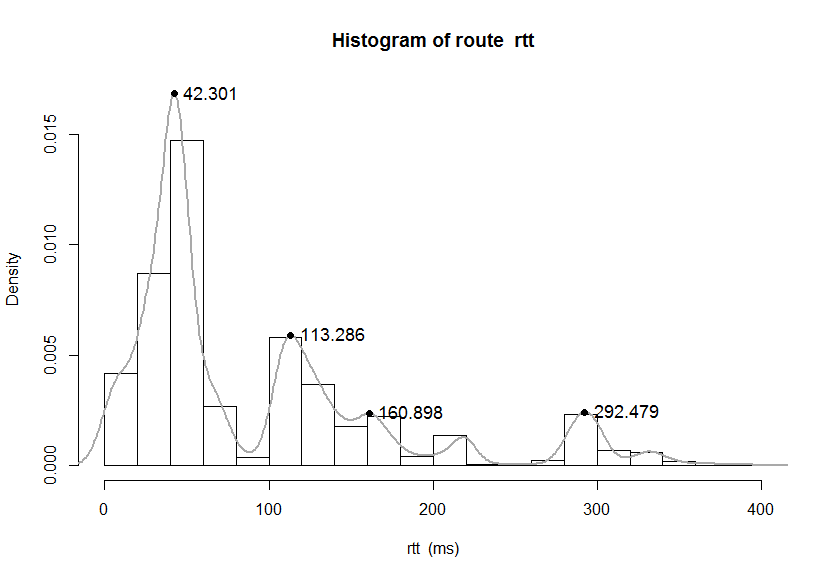
\includegraphics[width=0.95\textwidth, keepaspectratio]{figures/route_rtt_hist_max.png}
	\caption{Két végpont közötti késleltetés eloszlása}
	\label{fig:rtt-hist}
\end{figure}

A \ref{fig:rtt-hist} ábrán az egyik legalapvetőbb kimutatás látható, a késleltetések eloszlását a PlanetLab gépe között. Megfigyelhető az eloszlás lecsengése 350 milliszekundum felett, azonban a kimutatásból le lett vágva az rtt értékek felső 0.5\%-a. Ezek a mérések az esetek legnagyobb részében ideiglenes hálózati problémák alatt készültek, amelyek nem reprezentatívak a linkek tényleges tulajdonságaira vonatkozóan.

Az eloszlás első csúcsának elkülönülése a többitől az Internetet alkotó gráf útvonalainak a valós világhon alapuló tulajdonsága határozza meg. A mérési csomópontok túlnyomó része Európán vagy Amerikán belüliek, ezt magyarázza a 42 milliszekundum körüli első csúcs. Amint viszont egy kontinenseket átívelő linket érint a mérés, legalább 70 milliszekundumos késleltetés hozzáadódik az addigiakhoz, így adva a 113 milliszekundum körüli újabb csúcsot. A 70 milliszekundumos késleltetést a London-New York\footnote{Forrás: \href{https://wondernetwork.com/pings/New+York/London}{wondernetwork.com}} közötti tipikus késleltetés alapján lett figyelembe véve. A további késleltetés csúcsok további kontinensek közötti késleltetések alapján származtathatóak. Az hasonló kimutatások jól prezentálják az Internetnek a valós világunkhoz való szoros kapcsolatát.

Az rtt-ből származtatott delay adat az Internetet alkotó linkek és azok megfigyelhetőségére nyújt betekintést. Az útvonalakon lévő hálózati eszközök eltérő módon válaszolnak a lejárt TTL mezőjű adatcsomagokra, amelyeket a traceroute használ. Ennek legegyértelműbb bizonyítéka a delay adatsor kvantiliseinek értékei:

\renewcommand{\arraystretch}{1.3}
\begin{table}[ht]
	\centering
	\caption{A delay adatsor kvantilisei}
	\hspace{2mm}
	\begin{tabular}{ | c | c | c | c | c |}
	\hline
0\% & 25\% & 50\% & 75\% & 100\% \\ \hline
-2217.682 & -0.188 & 0.631 & 6.775 & 2323.324 \\ 
\hline
	\end{tabular}
	\label{tab:delay_kvant}
\end{table}

A \ref{tab:delay_kvant} táblázatból az olvasható le, hogy a delay értékeknek legalább 25\%-a negatív értékű és széles tartományon -2 szekundumtól +2 szekundumig terjed. A meglepően nagy arányban előforduló negatív értékek magyarázata az, hogy míg egy hálózati eszköz képességeinek megfelelően azonnal visszaküldi a lejárt TTL mezőjű csomagokat, addig egyes eszközök ezt késleltetve teszik meg.
Az adatsor eredeti hisztogramja nincs bemutatva, mivel egyetlen csúcs látszódna csak az origó környékén, a túlságosan szélsőséges értékek miatt.

\begin{figure}[h!]
	\centering
	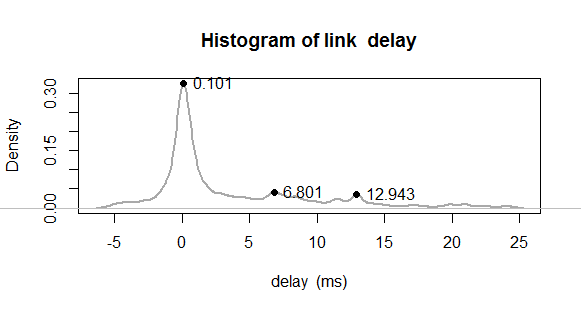
\includegraphics[width=0.95\textwidth, keepaspectratio]{figures/link-delay-dist.png}
	\caption{Két végpont közötti késleltetés eloszlása}
	\label{fig:link-delay}
\end{figure}

Az adatsornak ezért a két szélsőséges 5 percentilisét levágva készítettem el a valószínűségi változójának a sűrűségfüggvényét. Annak ellenére, hogy a linkekre becsült késleltetések többnyire 0,1 milliszekundum körül helyezkednek el az átlaguk 6,12 milliszekundum.

\pagebreak

\begin{figure}[h!]
	\centering
	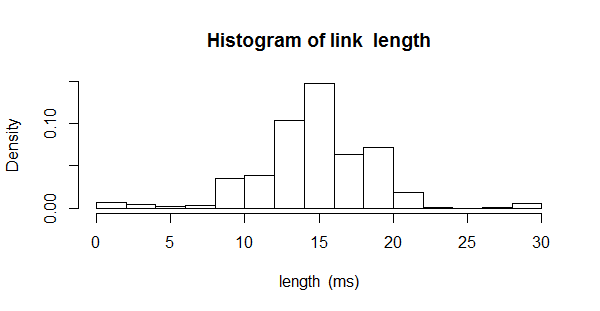
\includegraphics[width=0.95\textwidth, keepaspectratio]{figures/link-length-hist.png}
	\caption{Az útvonalak HOP számának eloszlása}
	\label{fig:link-len}
\end{figure}

Ellenőrzésként a mérésben résztvevő útvonalak késleltetése 93,3 milliszekundum átlagosan, a közbülső linkek száma pedig 15,3 átlagosan, ami igazolja a kimutatást. A linkek számáról részletesebb kimutatást a \ref{fig:link-len} ábra ad, amely a PlanetLab gépei közötti útvonalak HOP számának eloszlását mutatja.

A mérés legfőbb értékét az adja, hogy ezek a mérések nem egy hálózati pontból lettek indítva, hanem közel 200 csomópontból teljes hálót alkotva lettek elindítva a mérések. Ez olyan elemzésekre ad lehetőséget, mint az ú.n Hot-Potato jelenség megfigyelésére, amelyet korábbi kutatások is kimutatták\cite{hot-potato}.

\subsubsection*{A Hot Potato jelenség}

\begin{figure}[!ht]
	\centering
	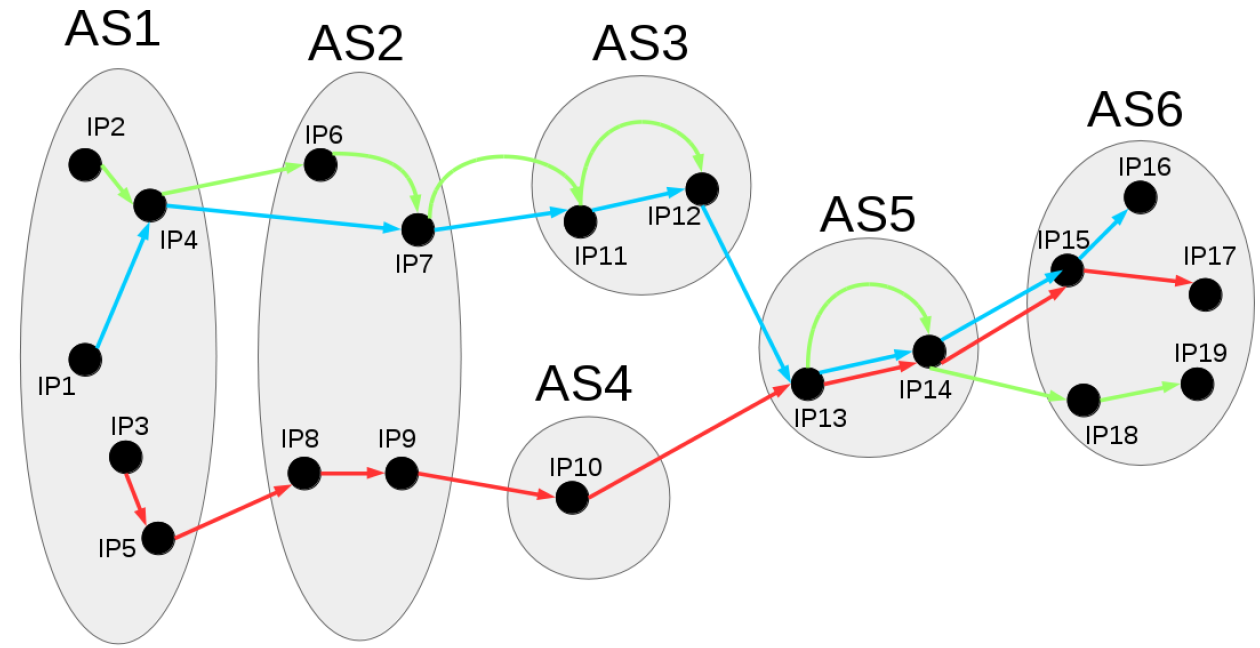
\includegraphics[width=0.7\textwidth, keepaspectratio]{figures/hot-potato.PNG}
	\caption{Csomagtovábbítási stratégia}
	\label{fig:hot-potato}
\end{figure}

\pagebreak

A \ref{fig:hot-potato} ábrán az látható, ahogy az AS1 ISP azonnal kivezeti a hálózatából a kék és piros küldendő adatcsomagot, hiába lettek azonos cél AS-hez címezve. A csomag továbbítása lefoglalná a saját erőforrásait. Ha más AS felé továbbítja, úgy mások erőforrásait használja. A szerződések ugyanis nem drágítják meg a csomagok továbbításának az árát, ha az távolabbra küldődik.

\begin{figure}[!ht]
	\centering
	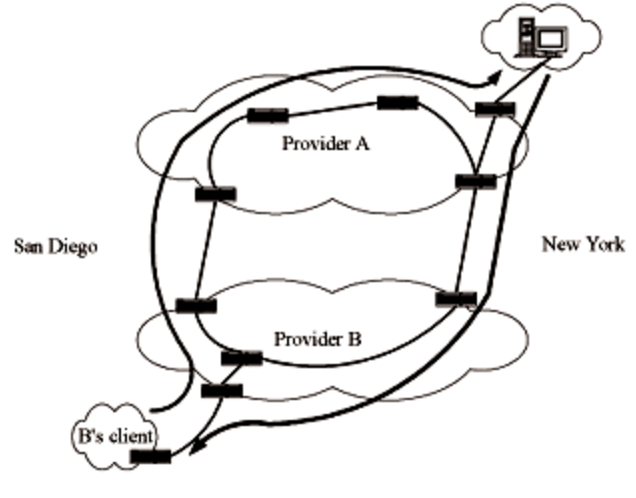
\includegraphics[width=0.4\textwidth, keepaspectratio]{figures/asymetric.PNG}
	\caption{Asszimetrikus útvonalválasztás a Hot-Potato jelenség miatt\protect\footnotemark}
	\label{fig:hot-potato}
\end{figure}

\footnotetext{Az ábra a \cite{hot-potato} forrásból lett átvéve}

A mérésekből úgy mutatható ki ez a stratégia, hogy azonos csomópont-pár esetén az egymás felé küldött csomagok nem feltétlen azonos útvonalon haladnak. Ugyanis a küldő ISP más útvonalat választ a hálózatából kifele küldött csomag számára, mint a fogadáskor.

\subsection*{PlanetLab gépek állapota}
A PlanetLab gépek eléréséről (az operációs rendszeréről) és hiba esetén a hibaüzenetek aggregált statisztikája. A következő adatokat tartalmazza:

\begin{itemize}
\item \textbf{erroneous:} Sikertelen csatlakozások száma (online gépek esetén)
\item \textbf{succeed:} Gépek száma, amelyeken sikeres volt a távoli parancsfuttatás (cat /etc/issue)
\item \textbf{online:} A ping parancssal elérhető gépek száma
\item \textbf{offline:} A ping parancssal nem elérhető gépek száma
\item \textbf{outputs:} Az összes különböző kimenet felsorolása a hozzá tartozó előfordulások számával.
\item \textbf{error\_types:} Az összes különböző hibatípus felsorolása a hozzá tartozó előfordulások számával
\item \textbf{ts:} A mérés időpontja
\end{itemize}

\begin{figure}[!ht]
	\centering
	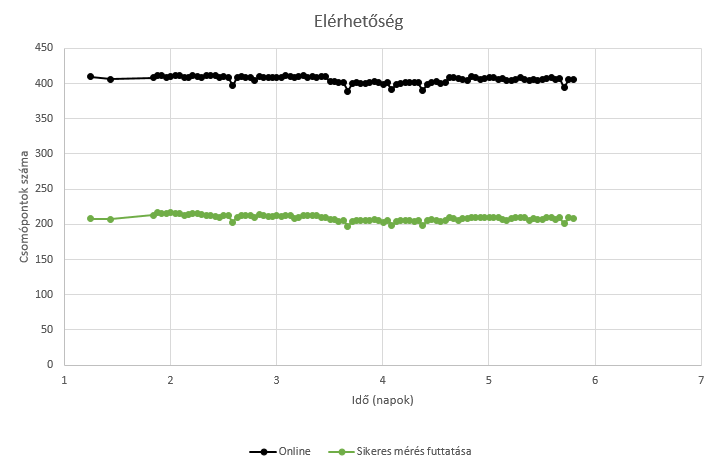
\includegraphics[width=0.9\textwidth, keepaspectratio]{figures/availability.PNG}
	\caption{A PlanetLab hálózat gépeinek elérhetősége egy hetes mintavételen}
	\label{fig:availability}
\end{figure}

Ez az adat kollekció a legfontosabb forrása a mérési rendszer rendelkezésre állásának és a hozzá szükséges PlanetLab hálózat elérhetőségének monitorozásának. A \ref{fig:availability} ábrán látható az online és a succeed adatsorok egy hetes mintavétele. Jól látható, hogy a PlanetLab hálózatának elérhetőségében van egy kevés fluktuáció, maximum 10 gép körüli szórással azonban összességében stabilan elérhetőek.



\subsection*{AS gráf él információi}
A korábban részletesen bemutatott AS gráf ezen kollekció adataiból lett felépítve:

\begin{itemize}
\item \textbf{asn:} A autonóm rendszer azonosító száma
\item \textbf{core\_ips:} Az autonóm rendszeren belül észlelt ip címek
\item \textbf{gateways\_to\_as:} Az autonóm rendszerből másikba vezető kapcsolatok listája. A másik AS-hez irányuló ip cím párok (egyik AS kimeneti címe, másik AS bemeneti címe) listáit is tartalmazza.
\end{itemize}



\begin{figure}[h]
	\centering
	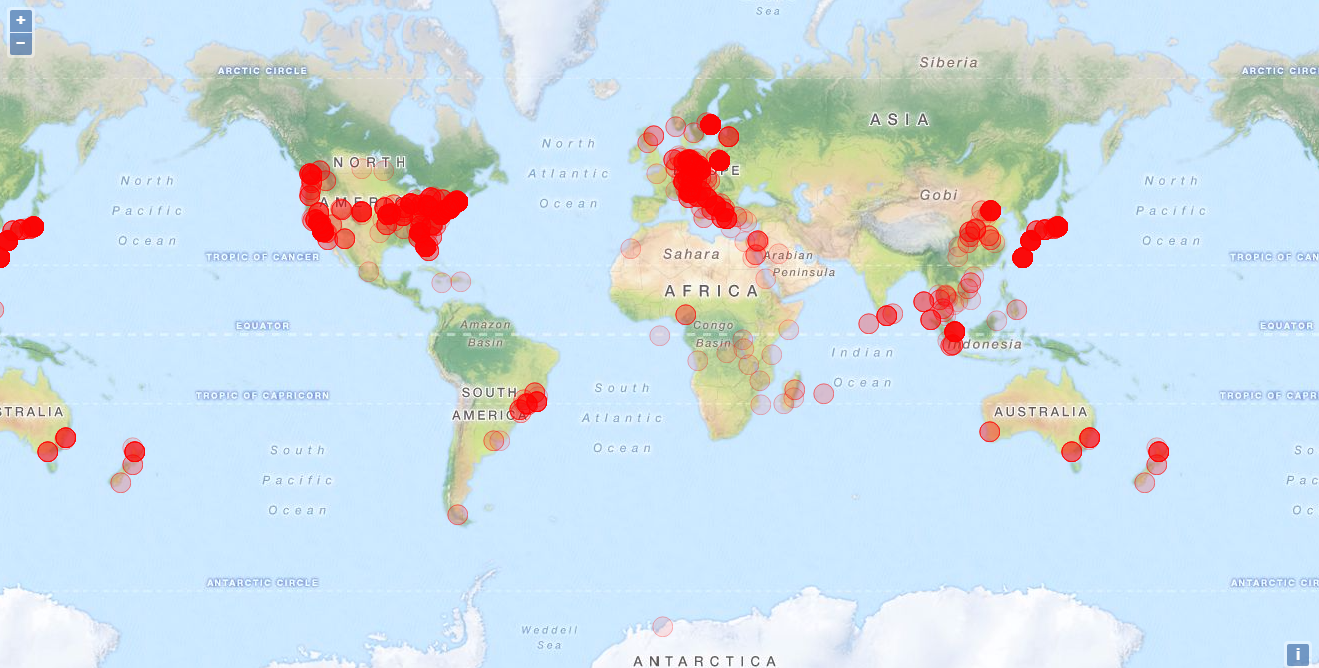
\includegraphics[width=0.9\textwidth, keepaspectratio]{figures/ip_map.png}
	\caption{A mérésben résztvevő ip címek geolokációs pozíciójai}
	\label{fig:ip-map}
\end{figure}

\section{Gráf ábrázolása}

Az gráf tulajdonságainak intuitív leolvasásához ábrázolások készültek. Mivel már egy mérés során több mint 1700 csomópontból álló gráfot kell ábrázolni, ezért ennek kivitelesése nehézségekbe ütközik. A \ref{fig:graph} ábrán látható egy ilyen gráf leképezés.

\begin{figure}[!ht]
	\centering
	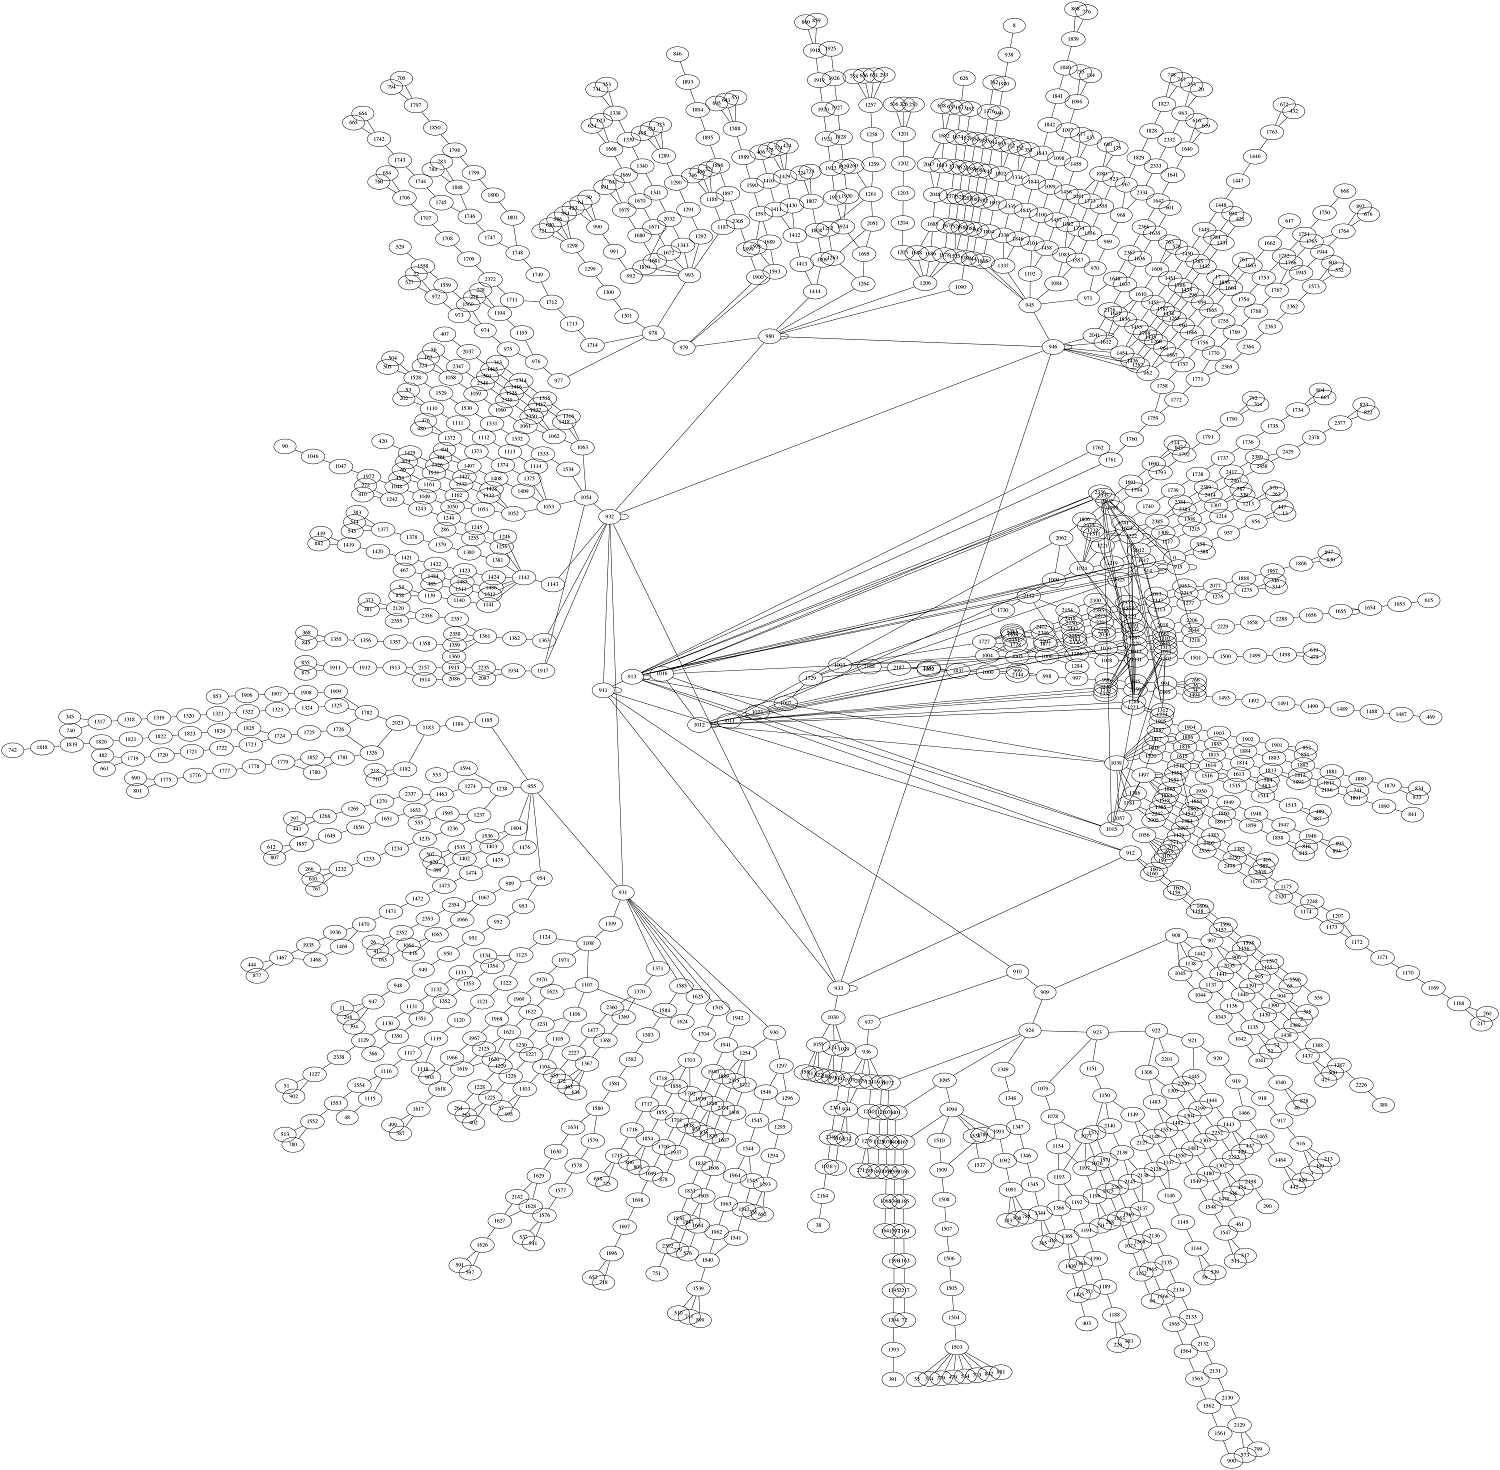
\includegraphics[width=1\textwidth, keepaspectratio]{figures/graph.png}
	\caption{Egy napi mérés gráfja az egyetem felé vezető útvonalak IP csomópontjaiból\label{fig:graph}}
\end{figure}

A \ref{fig:graph} ábrán jól láthatóak a középponttól távolodó hosszú fürtök, melyek egy cél IP cím AS-éhez vezető többnyire független útvonalakat reprezentálja.

\begin{figure}[h]
	\centering
	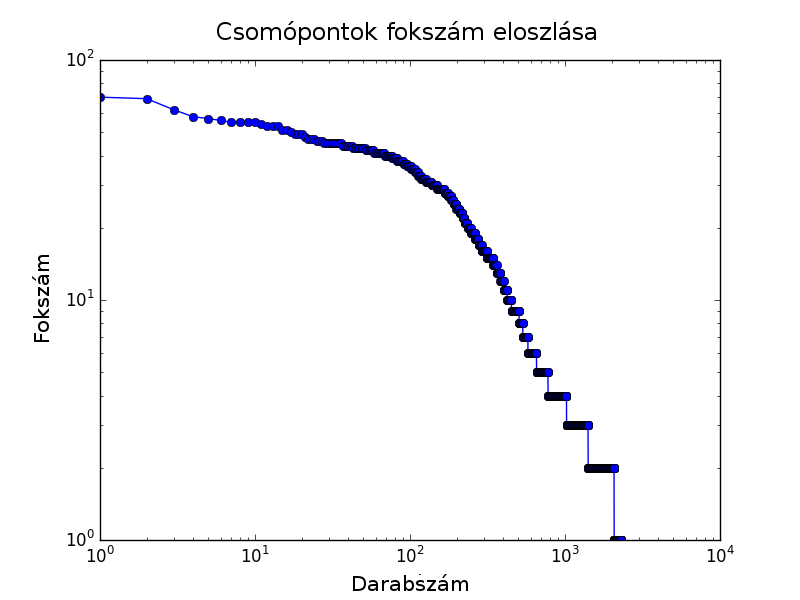
\includegraphics[width=0.95\textwidth, keepaspectratio]{figures/degree.png}
	\caption{A}
	\label{fig:ip-degree}
\end{figure}

\begin{figure}[h]
	\centering
	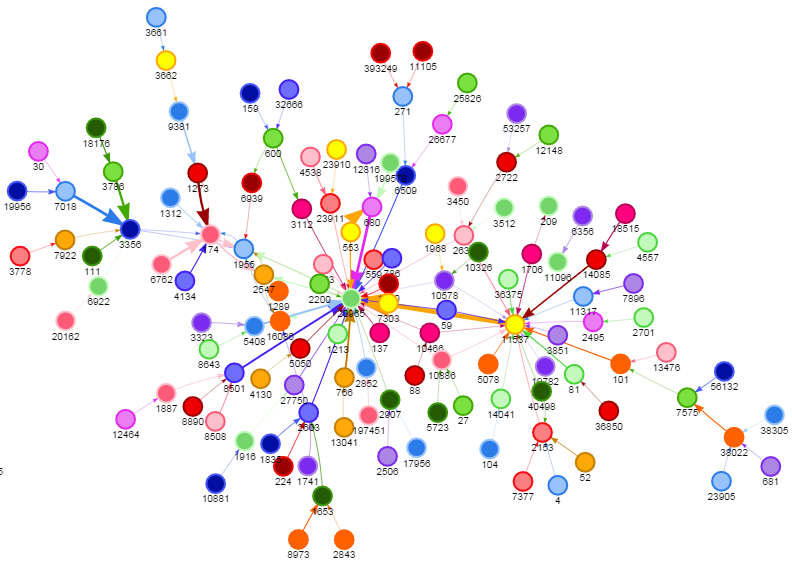
\includegraphics[width=0.95\textwidth, keepaspectratio]{figures/as-graph.png}
	\caption{A PlanetLab gépeitől az egyetem felé küldött csomagok által bejárt AS gráf}
	\label{fig:as-graph}
\end{figure}

Az AS szám információ felhasználásával a \ref{fig:as-graph} ábrán látható gráf lett elkészítve. Az ábra adatforrása pár nap folyamatos traceroute mérések eredménye. A PlanetLab csatlakozott gépeiről a BME egyik gépe felé címzett útvonalak lettek aggregálva. A nyilak vastagsága az alapján növekszik, hány különböző ip cím pár köti össze a két AS csomópontot. Ha minden átmenő csomag azonos ip címeken halad keresztül akkor az vékony lesz, míg ha két AS között haladó csomagok több különböző ip cím párokon keresztül utaznak az vastagabban van ábrázolva.

\begin{figure}[h]
	\centering
	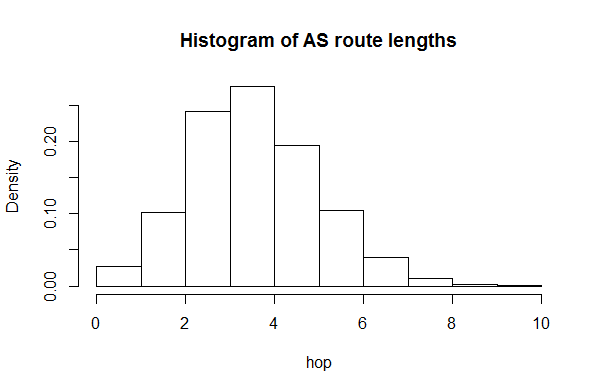
\includegraphics[width=0.9\textwidth, keepaspectratio]{figures/as-hop-hist.png}
	\caption{Az AS gráf csomópontjai között lévő útvonalak hosszának eloszlása}
	\label{fig:ip-map}
\end{figure}

A \ref{fig:as-graph} ábráról leolvasható hogy mely AS-ek kiterjedtek geolokációs tekintetben. Ha ugyanis több különböző ip útvonal köt össze két AS-t akkor azok valószínűleg területileg is több ponton vannak összeköttetésben.

A \ref{fig:as-graph} ábrán az összes útvonal a BME AS2547-es csomópontjába irányul, amely a valóságban kizárólag a AS1955-ös HBONE-AS HUNGARNET-tel van összeköttetésben. Egyes hibás traceroute mérések azonban torzítják ezt. A legnagyobb fokszámú csomópont az AS20965 , amely az AS1955 legfontosabb szomszédja, az elvi 17-ből\footnote{Forrás: Európai Regionális Internetes Nyilvántartó Hivatal honlapja: \href{https://stat.ripe.net/widget/asn-neighbours\#w.resource=1955}{stat.ripe.net}}.


\section{Middlebox felderítés}
A tanszéken végzett Internetes kutatásokhoz hozzáadott értéket jelentett a mérési rendszer. A kutatás középpontjában napjaink egyik Internetes trendje az úgynevezett Middlebox-ok voltak. Ez egy általános fogalom minden olyan hálózati eszközre vonatkozóan, amely beavatkozik és manipulálja a rajta átmenő forgalmat. Ilyen lehet a hagyományos tűzfal vagy terheléselosztó, de manapság újabb és újabb célra használják fel, néha beavatkozva a végpontok közötti kapcsolatba. Ez az Internet alapjait jelentő protokollok működésére akár nem kívánt hatással is lehet, ezért fontos kutatási téma napjainkban.

A kutatáshoz való hozzájárulása a mérési rendszernek az interneten küldött csomagok TTL mezőjének a manipulációját vizsgálta. Egy célgépen a tcpdump nevű alkalmazást volt elindítva olyan beállításokkal, hogy csak a mérésben résztvevő csomagokat vizsgálja. A PlanetLab hálózat elérhető gépein pedig speciálisan elkészített csomagok voltak küldve a célgép felé a maximális 250-es TTL mezővel. A vizsgálat a Middlebox-ok TTL manipulációját figyelte a különböző csomagtípusokra vonatkozóan.

Három csomagtípus manipulációja volt vizsgálva:

\begin{itemize}
\item \textbf{ICMP Ping request} Hagyományos ping üzenet kérési csomagja
\item \textbf{TCP SYN port:22} TCP kapcsolatfelépítési csomag a 22-es portra, amely az ssh kapcsolatok fogadására szolgál
\item \textbf{TCP SYN port:80} TCP kapcsolatfelépítési csomag a 80-as portra, amely a http kapcsolatok fogadására szolgál
\end{itemize}

A felhasznált parancsok a következők voltak:

\begin{lstlisting}[language=bash]
  # Celgepen futtatott parancs ICMP csomagok fogadasara
  sudo tcpdump -vnn -i eth0 icmp[icmptype] == 8 and dst host $ip
  # PlanetLab gepekrol kuldott ICMP csomagok parancsa
  ping -c 1 -t 250 $ip
  
  # A celgepen futtatott parancs TCP SYN csomagok fogadasara
  sudo tcpdump -vnn -i eth0 dst host $ip and "tcp[tcpflags] & (tcp-syn) != 0"
  # A PlanetLab gepeirol kuldott TCP csomagok parancsa
  nmap -v --ttl 250 --max-retries 1 -PS -p 80 $ip
  nmap -v --ttl 250 --max-retries 1 -PS -p 22 $ip
\end{lstlisting}


A mérés egy korábbi tanulmányt\cite{middlebox} vett alapul a felderítéshez. Az Internetes útvonalakon található, ttl mezőt manipuláló Middlebox-ok jelenlétét kimutatta a mérés. A mérés 75 szerverről küldött csomagok alapján lett elkészítve, mindegyik csomagtípusból egyet küldve a célgép felé, kivéve a 80-as portra küldöttek, amelyekből 3 csomag lett küldve gépenként.


\begin{figure}[!ht]
	\centering
	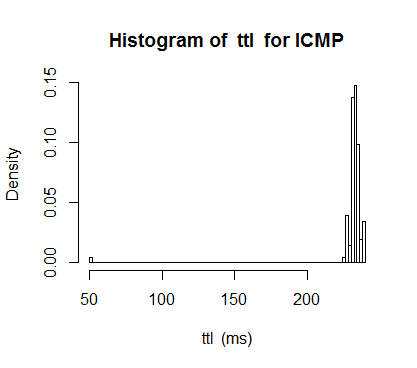
\includegraphics[width=0.3\textwidth, keepaspectratio]{figures/hist-ttl-icmp.png}
	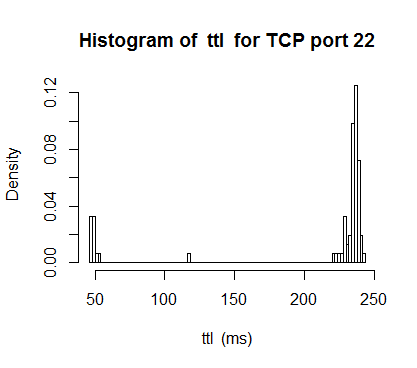
\includegraphics[width=0.3\textwidth, keepaspectratio]{figures/ttl-hist-22.png}
	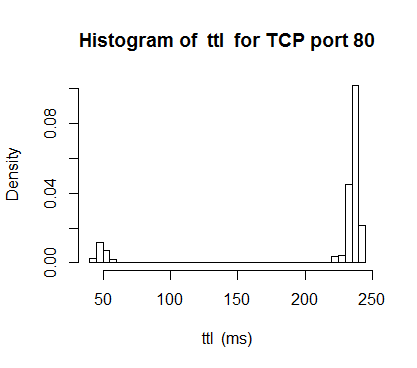
\includegraphics[width=0.3\textwidth, keepaspectratio]{figures/ttl-hist-port80.png}
	\caption{A fogadott csomagok TTL értékeinek előfordulási sűrűsége}
	\label{fig:ttl-hist}
\end{figure}

A \ref{fig:ttl-hist} ábrán látható, hogy az eredetileg 250-es TTL mezővel küldött csomagok egy része fogadáskor már egy közbülső elem által manipulálva lett. A manipuláció abból következtethető, hogy az útvonalak hosszúsága normális eloszlást követ, ahogy a \ref{fig:hop-hist} ábrán látható, valamint a TTL csökkenésnek függetlennek kellene lennie a csomag típusától.

\begin{figure}[!ht]
	\centering
	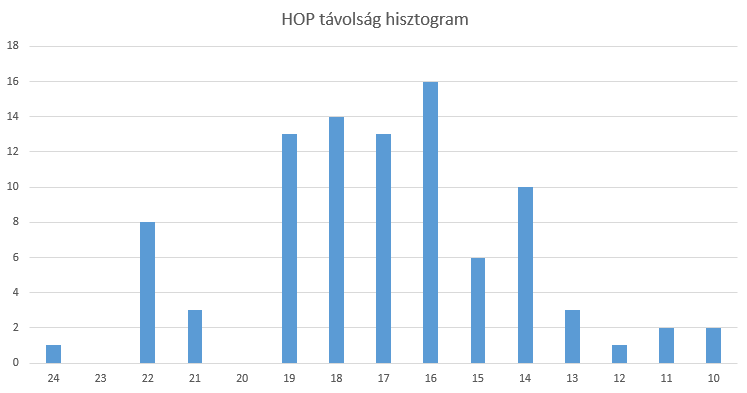
\includegraphics[width=0.5\textwidth, keepaspectratio]{figures/hop-hist.png}
	\caption{Az eredeti HOP távolsága a mért útvonalaknak}
	\label{fig:hop-hist}
\end{figure}

Az ICMP csomagok ábráján egyetlen csomag érkezett vélhetően módosított TTL mezővel, későbbi ellenőrzéskor azonban kiderült, egy nem a mérésben résztvevő gép küldte. A méréshez használt csomagszűrő minden Ping requestet átengedett, azonban a mérés ideje alatt a colorado-i egyetem egyik szervere is küldött ilyen csomagot, valószínűleg más Internetes mérés részeként. Ilyen módon kimondhatjuk, hogy az ICMP csomagok TTL mezője nem megy keresztül módosításon. Ezzel szemben a TCP csomagok, amelyeket vizsgáltunk az esetek több mint 10\%-ában módosításon estek keresztül. A 80-as portra küldöttek 11\%-a, míg a 22-es portra küldöttek 15\%-a. Itt megjegyzendő, hogy nem következetes az útvonalakon közbeiktatott manipuláció. Egyes útvonalakon csak a 22-es portra küldött csomagok lettek változtatva, másokon csak a 80-as portra küldöttek és természetesen legtöbb esetben mindkettő. Ezen felül a 80-as portra küldött 3 csomagból, manipuláció esetén a legtöbb esetben egyszerre voltak csökkentett TTL mezőjűek és érintetlenek is.

A vélhető ok, amiért az ICMP csomagokak érintetlenül hagyják a Middlebox-ok, az az ICMP csomagok hálózatdiagnosztikai természetéből adódik. Ezeket valószínűleg a hálózat helyes működésének ellenőrzéséhez is használják az operátorok. A hálózat egészséges működésének érdekében ezért támogatniuk kell az ICMP csomagok továbbításának a protokolloknak megfelelő módját.

Ez a mérés jól mutatja be a mérési rendszerben rejlő potenciált. A PlanetLab hálózatnak köszönhetően, az Internetre reprezentatív eredmények jöhetnek létre a gyorsan összeállítható mérési forgatókönyveknek hála.